\documentclass{VUMIFInfKursinis}
\usepackage{algorithmicx}
\usepackage{algorithm}
\usepackage{algpseudocode}
\usepackage{amsfonts}
\usepackage{amsmath}
\usepackage{bm}
\usepackage{color}
\usepackage{tikz}
\usepackage{enumitem}
% \usepackage{hyperref}  % Nuorodų aktyvavimas
\usepackage{url}

\setenumerate{topsep=0pt,itemsep=-1ex,partopsep=1ex,parsep=1ex}
\setitemize{topsep=0pt,itemsep=-1ex,partopsep=1ex,parsep=1ex}

% Titulinio aprašas
\university{Vilniaus universitetas}
\faculty{Matematikos ir informatikos fakultetas}
\department{Programų sistemų katedra}
\papertype{Kursinis darbas}
\title{Gestų kalbos atpažinimas naudojant internetinę kamerą}
\titleineng{Sign language recognition using web camera}
\status{3 kurso I grupės studentas}
\author{Pranciškus Ambrazas}
\supervisor{asist. Linas Petkevičius}
\date{Vilnius, \the\year}

% Nustatymai
% \setmainfont{Palemonas}   % Pakeisti teksto šriftą į Palemonas (turi būti įdiegtas sistemoje)
\bibliography{bibliografija} 

\begin{document}
\maketitle

\tableofcontents

\sectionnonum{Įvadas}

Daugiau nei 360 milijonų žmonių pasaulyje kenčia dėl klausos ir kalbos įvairių problemų, o daugiau nei 32 milijonai jų yra vaikai ir šis skaičius vis auga \cite{WhoInt}. Gestų kalba yra pagrindinis šių žmonių bendravimo įrankis. Tačiau reiktų pastebėti ir tai, jog dalis jų moka dalinai skaityti iš lūpų. 

Norint žmogui be šių ydų bendrauti su gestakalbiu (\textit{gestų kalba kalbantis žmogus}), o kartais net dviems gestakalbiams tarpusavyje, reikia vertėjo, kuris išverstų gestų kalbą į įprastinę ir atvirkščiai.

Kiekviena pasaulyje esanti kalba turi ir savo gestų kalbą. Tai reiškia, skiriasi tiek gestų kalbos gramatika, tiek netgi patys gestai. Pasaulyje randama net dialektų pagal regionus, ne tik pagal šalis. Amerikiečių anglų gestų kalba (\textit{toliau - ASL}) šnekančių žmonių pasaulyje priskaičiuojama nuo 500 tūkstančių iki netgi 2 milijonų vien tik Jungtinėse Amerikos Valstijose. Remiantis Census Bereau surinktais duomenimis, kuris domisi kalbų mažumomis, ASL yra pirmoji mažumos kalba, po „didžiojo ketverto“, kurį sudaro ispanų, italų, vokiečių ir prancūzų kalbos \cite{GUL}. Tad netgi bendraujant dviem žmonėms, mokantiems gestų kalbą neretai iškyla vertimo problema, todėl tenka ieškoti gestų vertimų. Paiešką šiuo metu galima atlikti atsižvelgiant į delno padėtį, vienos ar abiejų rankų judesį, jų padėtį ir gestą atliekančių rankų skaičių. Tuomet pagal gesto išvaizdos nuotraukas ar kartais net vaizdo įrašus, gestakalbiai gali išsiversti gestus. Tam yra skirtos tiek internetinės svetainės - žodynai, tiek įvairūs rašytiniai žodynai.


\subsectionnonum{Darbo tikslas}

Šio tyrimo tikslas - ištirti ir išanalizuoti galimybes internetinės kameros pagalba versti gestų kalbą, taip padedant ne tik gestakalbiams tarpusavyje, bet ir žmonėms, nesuprantantiems gestų kalbos bendrauti su gestakalbiais tam pasitelkiant technologijas. Galiausiai, taip suteikiant šiems žmonėms pilnavertį gyvenimą bendraujant su kitais. Šiuo tyrimu siekiama apžvelgti ir įvertinti ar naudojantis įprasta internetine kamera įmanoma paversti gestų kalbą rašytiniu tekstu ar net garsine kalba ir lygiai taip pat versti rašytinę ar garsinę kalbą į gestų kalbą. Taip pat siekiama apžvelgti ar įmanoma sukurti visiems gestakalbiams prieinamą produktą ar programinę įrangą, kurią kiekvienas įsidiegęs į savo įrenginį - kompiuterį, mobilųjį telefoną ar planšetinį kompiuterį - galėtų naudotis šiuo vertėju. Vėliau tai galėtų tapti ir mokomąja gestų kalbos priemone. 
%Šiuo metu yra gaminamas vienas iš tokių produktų, tačiau tai yra atskiras įrenginys, turintis įmontuotą kamerą, kuri be vaizdo taip pat fiksuoja ir atstumą iki tam tikrų objektų (šiuo atveju rankos), tačiau produkto kūrėjai sako, jog jų įrenginys galės versti gestų kalbą į anglų ir kitas kalbas ir lygiai taip pat versti įprastą kalbą į rašytinę kalbą. Plačiau: \textit{http://www.motionsavvy.com/}

\subsectionnonum{Naudojamos priemonės}
\begin{enumerate}
	\item Programavimo kalba Python;
	\item Vaizdų apdorojimo įrankis OpenCV;
	\item Matematinių skaičiavimų biblioteka NumPy;
	\item Įrankių moksliniams tyrimams biblioteka SciPy;
	\item Savaime apmokomų sistemų biblioteka scikit-learn;
	\item Neuroninių tinklų aplikacijų programavimo sąsaja Keras;
	\item Atviro kodo skaičiavimo operacijų biblioteka TensorFlow, kuri labiausiai specializuojasi ties apsimokančiomis sistemomis;
	\item Įrankis Docker.
\end{enumerate}

\subsectionnonum{Tyrimo eiga}
Šiame darbe bus nagrinėjama amerikiečių anglų ir lietuvių gestų kalbos.
\begin{enumerate}
	\item Susipažinimas su gestų kalba ir jos problematika;
	\item Susipažinimas su kelių tipų apmokomomis sistemomis;
	\item Praktinis pritaikymas.
\end{enumerate}

%Įvade apibūdinamas darbo tikslas, temos aktualumas ir siekiami rezultatai.
%Darbo įvadas neturi būti dėstymo santrauka. Įvado apimtis 1–2 puslapiai.

\section{Teorija}
Šiame skyriuje bus aprašoma teorija apie apmokomas sistemas ir neuroninius tinklus.

\subsection{Apmokomos sistemos}

\textbf{Apmokomos sistemos} (\textit{angl. machine learning}) – tai mokslas apie tai, kaip kompiuterius užprogramuoti taip, jog jie patys darytų sprendimus be žmogaus įsikišimo neužprogramuojant kiekvienos galimos situacijos. Kitais žodžiais tariant, leisti kompiuteriui pačiam nuspręsti kaip elgtis esant tam tikroms aplinkybėms. Apmokomos sistemos yra didelis žingsnis į priekį norint sukurti dirbtinį intelektą.

Apmokomų sistemų ir jų algoritmų sukūrimo dėka gatvėmis pradėjo važinėti patys save vairuojantys automobiliai (\textit{angl. self-driving cars}) arba dar kitaip vadinamos autonominės transporto priemonės. Įvairūs paieškos varikliai tokie kaip „Google“ ar „Yahoo“ taikydami šiuos alogirtmus naudotojams rodo kiekvienam asmeniškai sugeneruotą turinį. Taip pat reikėtų paminėti ir kalbos atpažinimo sistemas tokias kaip „Siri“ ar „Google Assistant“, kurios iš joms duotų komandų atlieka tam tikrus veiksmus.

\subsection{Neuroniniai tinklai}
\textbf{Neuronas} (\textit{arba - nervinė ląstelė}) – pagrindinės nervų sistemos ląstelės, sukuriančios ir/arba perduodančios elektrocheminius impulsus.



Žmogaus smegenys yra sudėtingas, nelinijinis ir paralelinis kompiuteris\cite{Hay09}, kurias sudaro neuronai. Vienas neuronas vienu metu jungiasi su daugybe kitų neuronų per dendritus, ant kurių yra daug sinapsių, per kurias ateina informacija iš kitų neuronų. Dendritus paprasčiau galima pavadinti kaip informacijos prięmėjais. Todėl vienas neuronas gali sudaryti iki 100000 sinapsių. Kiekviena sinapsė gali būti jaudinanti arba slopinanti. Visas šis mechanizmas dar nadinamas \textbf{neuroniniu tinklu} (\textit{angl. Neural network}).

Vienas neuronas priima informaciją per dendritus, tuomet pats neuronas nusprendžia ar bus siunčiama informacija į kitus neuronus ir kokia ji bus siunčiama (\textit{žr. \ref{img:neuron_structure} pav.})

\begin{figure}[H]
	\centering
	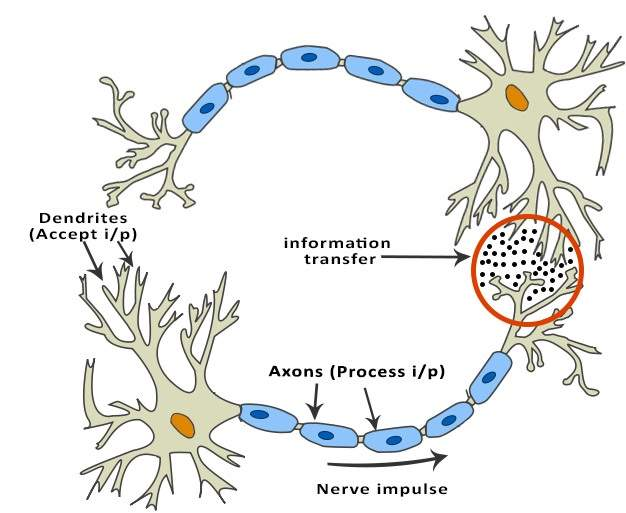
\includegraphics[width=.5\linewidth]{img/neuron-structure}
	\caption[]{Neuroninio tinklo struktūra\footnotemark}
	\label{img:neuron_structure}
	%https://www.tutorialspoint.com/artificial_intelligence/artificial_intelligence_neural_networks.htm
\end{figure}
\footnotetext{\url{https://www.tutorialspoint.com/artificial_intelligence/artificial_intelligence_neural_networks.htm/}}

Remiantis šiais principais buvo sukurti dirbtiniai neuroniniai tinklai.


\subsubsection{Dirbtiniai neuroniniai tinklai}
\textbf{Dirbtinis neuroninis tinklas} (\textit{angl. Artificial neural network}) – struktūra, skirta apdoroti dideliam kiekiui informacijos, sukurta rementis žmogaus nervų sistemos veikimo principu. Kitais žodžiais tariant, skaitmenizuota žmogaus smegenų veikla.

Neuronai dirbtiniame neuroniniame tinkle yra sujungti jungtimis. Taip jie tarpusavyje komunikuoja perduodami vienas kitam informaciją. Kiekvienas neuronas gali priimti atėjusią informaciją, ją apdoroti ir perduoti kitam neuronui. Kiekviena jungtis turi savo svorį, pagal kurį pasirenkama, į kurį neuroną turi būti perduodama informacija toliau. Šių jungčių svorius galime įvertinti naudodamiesi apmokomų sistemų pagalba. 

\ref{fig:ann} pav. pateikiama supaprastinta schema, kaip veikia dirbtiniai neuroniniai tinklai:

\begin{figure}[H]
	\centering
	\tikzset{%
		every neuron/.style={
			circle,
			draw,
			minimum size=1cm
		},
	}
	
	\begin{tikzpicture}[x=1.5cm, y=1.5cm, >=stealth]
	\centering
	
	\foreach \m/\l [count=\y] in {1,2,3}
	\node [every neuron/.try, neuron \m/.try] (input-\m) at (0,1.9-\y) {};
	
	\foreach \m [count=\y] in {1,2,3,4}
	\node [every neuron/.try, neuron \m/.try ] (hidden-\m) at (2,2.5-\y) {};
	
	\foreach \m [count=\y] in {1,2}
	\node [every neuron/.try, neuron \m/.try ] (output-\m) at (4,2.3-\y*1.6) {};
	
	\foreach \i in {1,...,3}
	\foreach \j in {1,...,4}
	\draw [->] (input-\i) -- (hidden-\j);
	
	\foreach \i in {1,...,4}
	\foreach \j in {1,...,2}
	\draw [->] (hidden-\i) -- (output-\j);
	
	\foreach \l [count=\x from 0] in {Įeigos, Paslėptasis, Išeigos}
	\node [align=center, above] at (\x*2,2) {\l \\ sluoksnis};
	\end{tikzpicture}
	\caption{Dirbtinio neuroninio tinklo pavyzdys} \label{fig:ann}
\end{figure}

\subsubsection{Konvoliuciniai neuroniniai tinklai}
\textbf{Konvoliuciniai neuroniniai tinklai} (\textit{angl. Convolutional neural network}) (\textit{toliau - KNT}) – specilios rūšies „Feed-forward“ neuroniniai tinklai, kurie reamiasi tuo pačiu dirbtinių neuroninių tinklų (\textit{žr. \ref{fig:ann} pav.}) principu. Šie tiklai yra skirti atpažinti objektus. Apmokant KNT, pagrindinis principas, kaip ir raktinis šių tinklų žodis, yra konvoliucija. Tai tarsi filtrai, kurie išskaido kadrą į dalis, pritaiko įvairius filtrus ir gliausiai randa pasikartojančius įvairiuose kadruose esančius požymius. Tokius kaip ratas, langai ar pan., o šio tyrimo atveju - rankos, delnai, pirštai, jų padėtis ir kt.

Šiame tyrime bus pasinaudota ReLU principu nes konvoliuciniai neuroniniai tinklai, kurie remiasi ReLU principu yra kelis kartus greitesni, nei tie, kurie remiasi kitais principais, pavyzdžiui, \textit{tanh} \cite{NIPS2012_4824}. 

Kuomet kadrui yra pritaikoma konvoliucija (sudauginami visi kadro taškai su konvoliucine matrica), pritaikomas ReLU principas, kuris visus neigiamus skaičius paverčia į 0. Telkimo (\textit{angl. pooling}) fazėje, kadras yra sumažinamas (\textit{žr. \ref{img:cnn} pav.}). Plačiau šie etapai bus aptarti 3.3 skyriuje.

\begin{figure}[H]
	\centering
	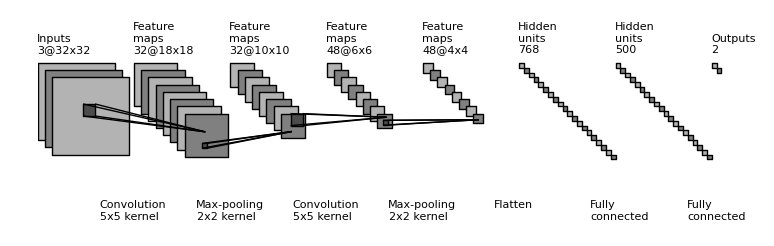
\includegraphics[width=.8\linewidth]{img/cnn}
	\caption[]{Konvoliucinių neuroninių tinklų schema\footnotemark}
	\label{img:cnn}
\end{figure}
\footnotetext{\url{http://yann.lecun.com/exdb/lenet/}}


\subsubsection{Rekurentiniai neuroniniai tinklai}
\textbf{Rekurentiniai neuroniniai tinklai} (\textit{angl. Recurrent neural network}) – tai dirbtinis neuroninis tinklas, kuris saugo informaciją apie praeituose žingsniuose (neuronuose) atliktus veiksmus ar skaičiavimus. Remiantis rekurentinių tinklų savybe galima naudoti jau surinktą informaciją, o šiuo atveju tai labai pasitarnautų, kuomet gestas nėra statinis. Todėl kiekviename kadre jeigu fiksuojama kažkokio statinio gesto reikšmė, tai sujungus jas į rekurentinį neuroninį tinklą galima atpažinti dinaminius gestus.


\begin{figure}[H]
	\centering
	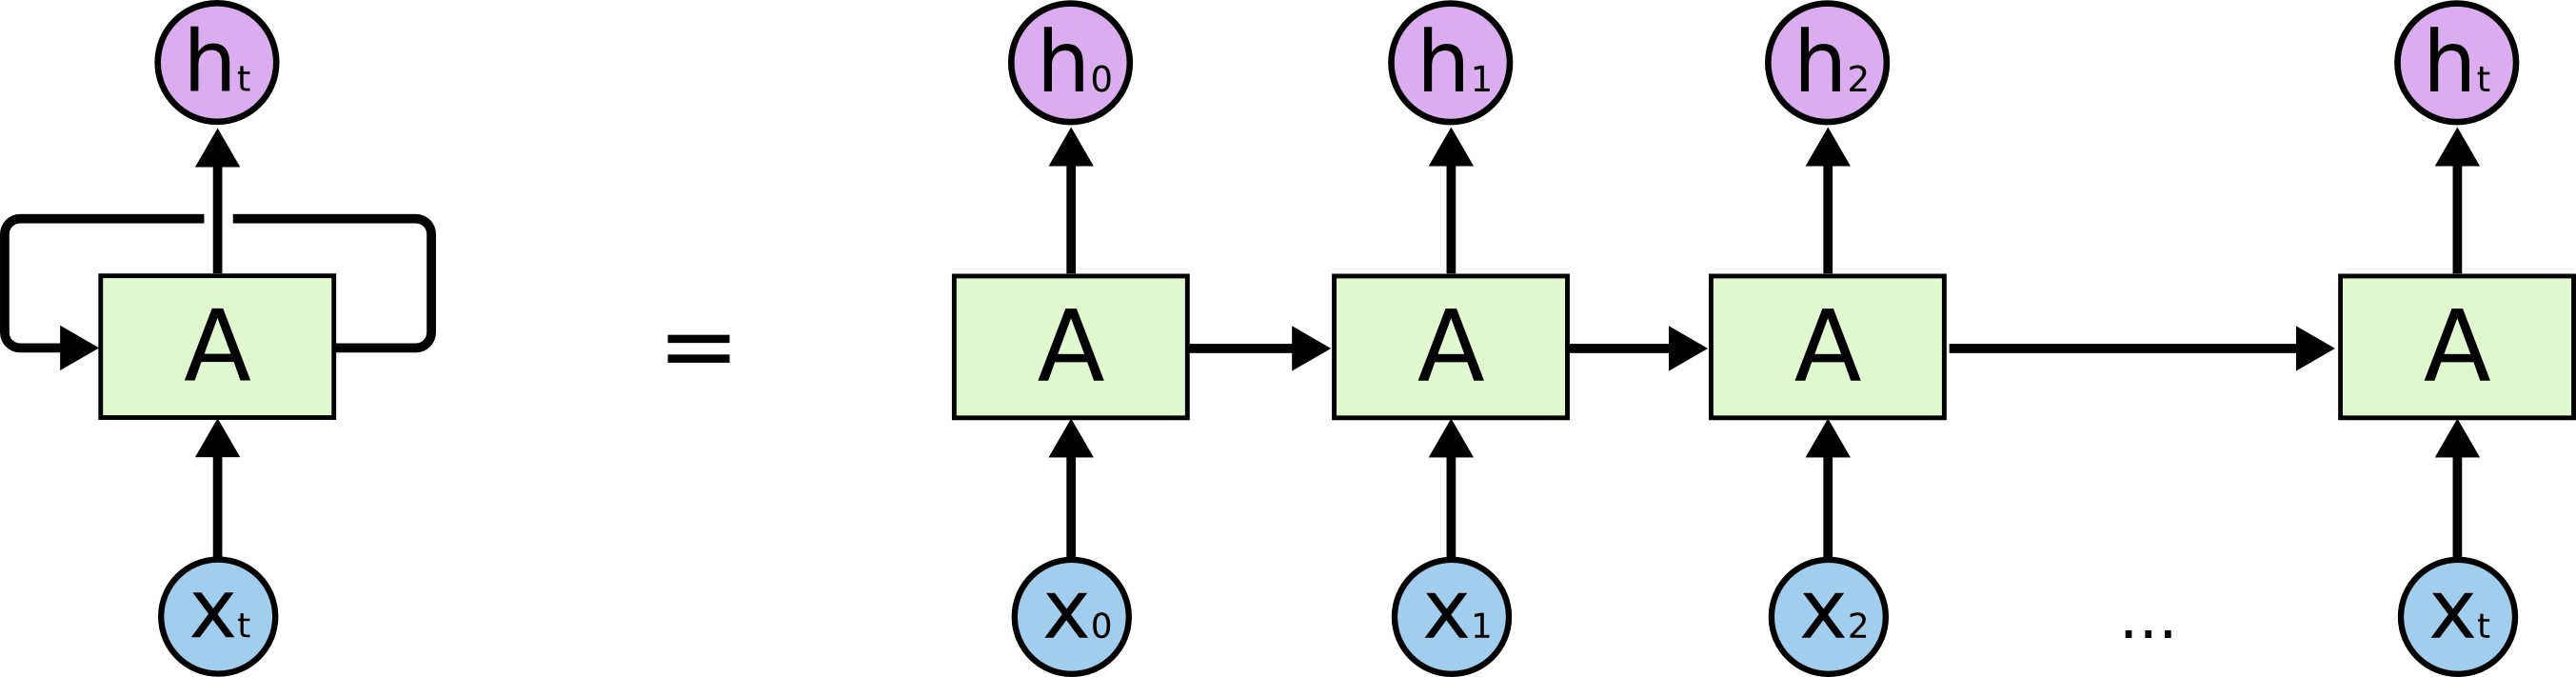
\includegraphics[width=.8\linewidth]{img/rnn}
	\caption[]{Rekurentinių neuroninių tinklų schema\footnotemark}
	\label{img:rnn}
\end{figure}
\footnotetext{\url{http://colah.github.io/posts/2015-08-Understanding-LSTMs/}}
\begin{itemize}
	\item \textit{x\textsubscript{t}} - įeiga momentu \textit{t};
	\item \textit{h\textsubscript{t}} - išeiga momentu \textit{t};
	\item \textit{A\textsubscript{t}} - būsena momentu \textit{t}.
\end{itemize}


\section{Gestų kalba}
\subsection{Gestų kalbos skirstymas}
Gestų kalba susideda iš dviejų dalių – statinių ir dinaminių ženklų. Gestų kalboje kiekviena kalba turi savo abėcėlę. Statiniais ženklais atvaizduojama didžioji abėcėlių raidžių dalis bei kai kurie žodžiai. O dinaminiais - didžioji dalis žodžių ir kai kurios gestų abėcėlių raidės. \textit{Pavyzdžiui}, amerikiečių gestų kalbos abėcėlėje J ir Z raidės atvaizduojamos dinaminiais judesiais (\textit{žr. \ref{img:asl_alphabet} pav.}), o lietuvių - jau minėtosios J ir Z raidės bei Ą, D, Į, K ir kt. (\textit{žr. \ref{img:lsl_alphabet} pav.})


\begin{figure}[H]
	\centering
	\begin{minipage}{.5\textwidth}
		\centering
		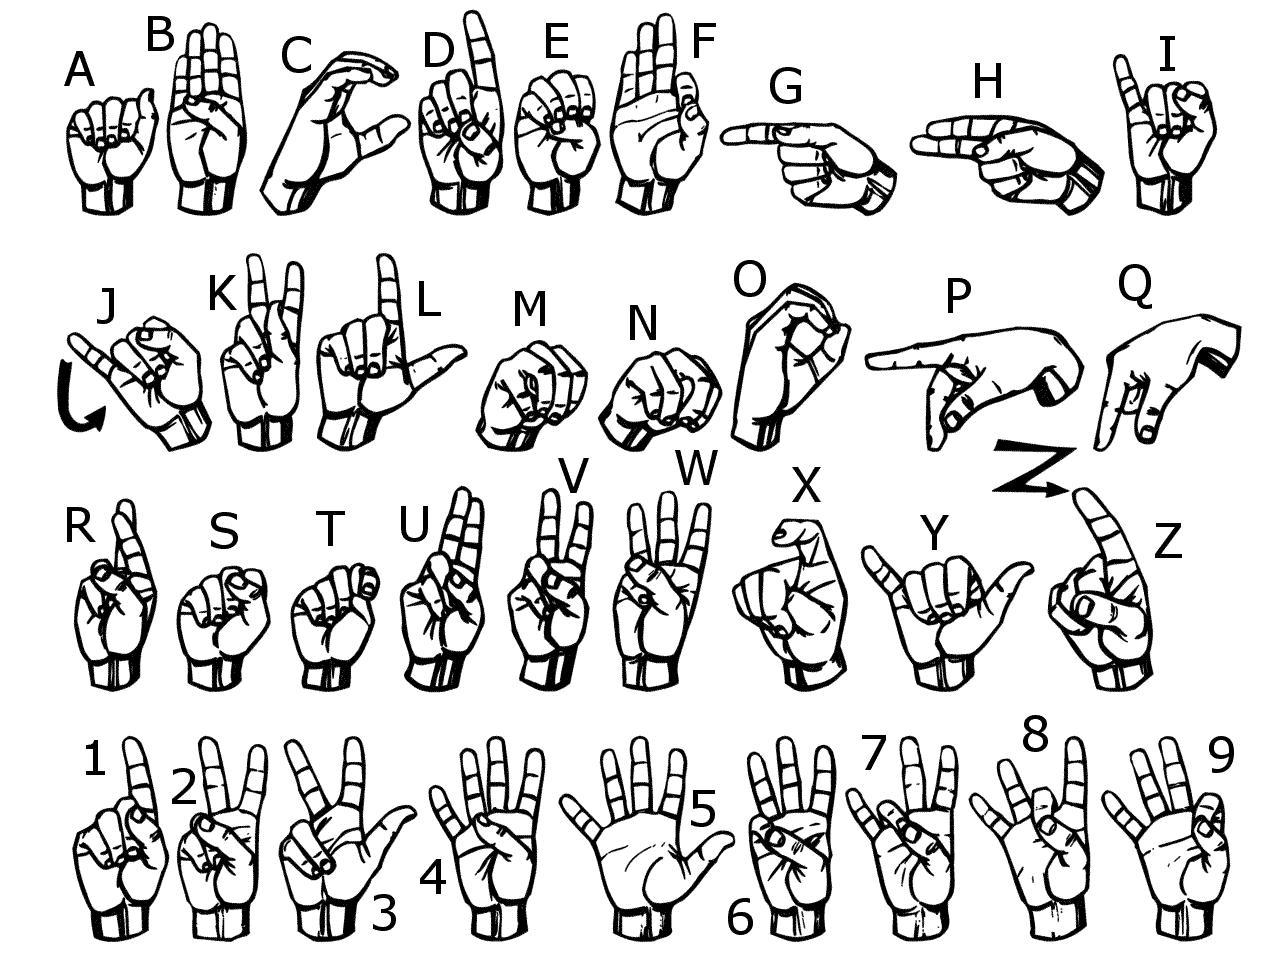
\includegraphics[width=.8\linewidth]{img/asl_alphabet}
		\caption[a]{Amerikiečių gestų kalbos abėcėlė\footnotemark}
		\label{img:asl_alphabet}
	\end{minipage}%
	\begin{minipage}{.5\textwidth}
		\centering
		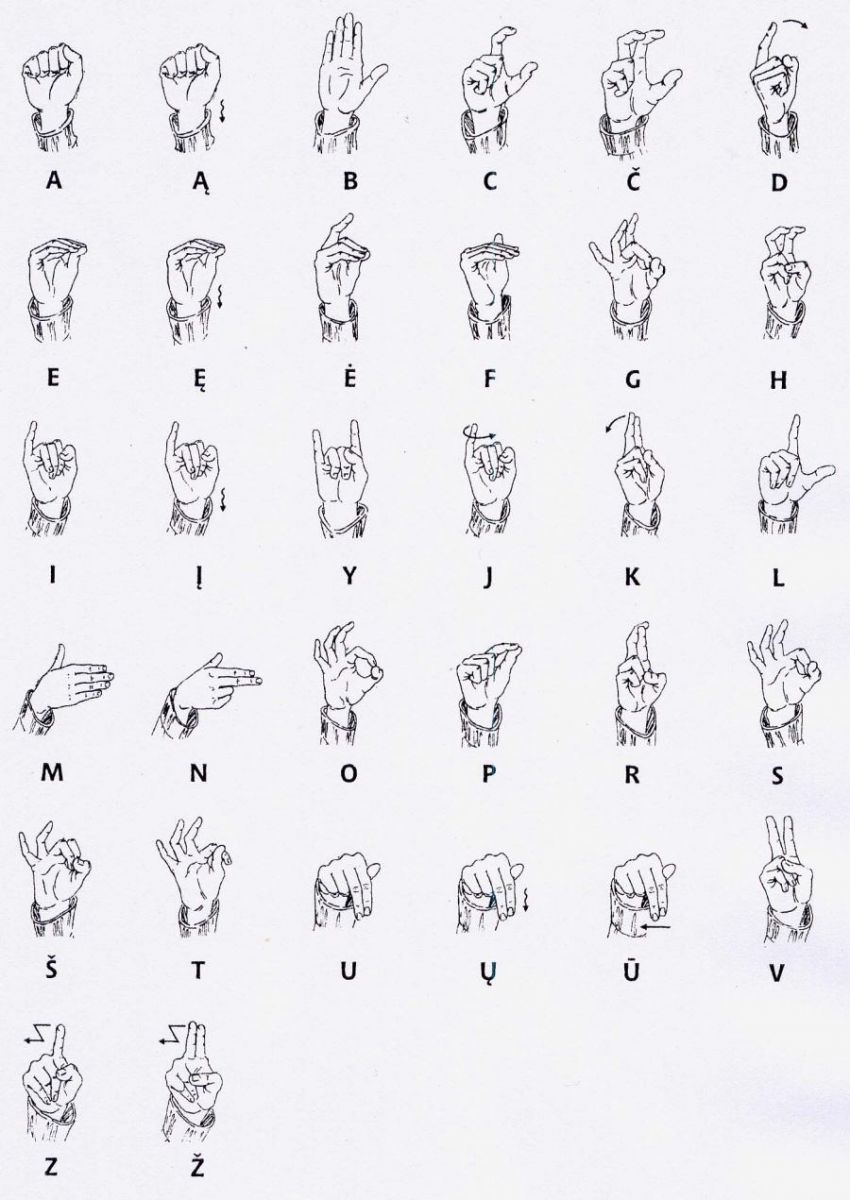
\includegraphics[width=.5\linewidth]{img/lsl_alphabet}
		\caption[b]{Lietuvių gestų kalbos abėcėlė\footnotemark}
		\label{img:lsl_alphabet}
	\end{minipage}
\end{figure}
\footnotetext[4]{\url{http://lifeprint.com/asl101/topics/wallpaper1.htm}}
\footnotetext{\url{http://gestai.ndt.lt/pirstu-abecele}}
\subsection{Problematika}
Norint atpažinti gestus, paversti juos į raides, žodžius ar sakinius susiduriama su problemomis, kurios susijusios tiek su statinių, tiek su dinaminių gestų atpažinimu.

\subsubsection{Statinių ženklų problematika}
Pagrindinės problemos iškylančios atpažįstant statinius gestų kalbos ženklus yra:
\begin{enumerate}
	\item Kiekvienos kalbos abėcėlę sudaro skirtingas statinių ženklų skaičius. \textit{Pavyzdžiui}, lietuvių kalbos abėcėlę sudaro 32 ženklai, o amerikietišką - 26; 
	\item Kiekvienoje kalboje skiriasi statinių ženklų skaičius ir jais atvaizduojamos raidės ar žodžiai. \textit{Pavyzdžiui}, abėcėlių raidžių skirtumai;
	\item Gestų panašumai. \textit{Pavyzdžiui}, raidės A, E, N, S, T yra atvaizduojamos sugniaužtus kumštį, o net trijose iš jų (A, E ir S) skiriasi tik nykščio padėtis;
	\item Kampas, kuris susidaro atpažįstant gestą. \textit{Pavyzdžiui}, kai A raidė rodoma ne iš priekio, o iš šono;
	\item Apšvietimas. \textit{Pavyzdžiui}, gestų atpažinimas esant prieblandai ir dienos šviesai.
\end{enumerate}
\subsubsection{Dinaminių ženklų problematika}
Pagrindinės problemos iškylančios atpažįstant dinaminius gestų kalbos ženklys yra:
\begin{enumerate}
	\item Nauji gestų kalbos žodžiai. \textit{Pavyzdžiui}, kiekvienas uraganas turi savo pavadinimą, todėl tai gali reikšti naujo gesto atsiradimą; 
	\item Gesto kelios reikšmės. \textit{Pavyzdžiui}, vienas gestas gali turėti kelias reikšmes, kaip kad lietuvių kalboje vienas žodis „kasa“ gali turėti net tris skirtingas reikšmes;
	\item Kampas, kuris susidaro atpažįstant gestą. \textit{Pavyzdžiui}, kai rodantysis žmogus stovi šiek tiek šonu;
	\item Žodžių apjungimas į vieną sakinį. \textit{Pavyzdžiui}, keli gestai einantys vienas po kito gali reikšti kelis žodius, tačiau tuo pačiu būti panašūs į vieną gestą, kuris jau reikš tik vieną žodį.
\end{enumerate}

\section{Sistemos apmokymas}
Norint, jog sistema atpažintų gestus, svarbiausia ją apmokyti, ką reiškia tam tikri gestai. Tam galime išnaudoti kadrus (\textit{angl. frame}) ir apmokomų sistemų galimybes. Šiame skyriuje bus aptarta, kaip apmokyti sistemą atpažinti statinę ASL abėcėlę.

\subsection{Kadro transofrmacija}
Kiekvienas kadras yra sudarytas iš (\textit{h, w, c}) taškų (\textit{angl. pixels}). Čia, \textit{h} - aukštis (\textit{angl. height}), \textit{w} - plotis (\textit{angl. width}), \textit{c} - spalva (\textit{angl. color}), susidedanti iš RGB spalvų paletės. RGB spalvų paletė – trijų (raudonos, žalios ir mėlynos) spalvų paletė, kuri yra ypatinga tuo, jog kiekviena spalva, kurią mato žmogus, susideda būtent iš šių trijų spalvų, varijuojant jų ryškumu. 0 - spalva nenaudojama, o 255 - spalva naudojama pilnai ryškiai. Tad kiekvieną kadrą galima išskirti į šių trijų spalvų sluoksnius.

\subsection{Sistemos apmokymas, naudojantis įprastinėmis sistemomis}
\textbf{Kompiuterio vaizdų atpažinimo sistemos} (\textit{angl. computer vision}) – sistemos, kurias galima apmokyti atpažinti įvairius objektus, dar žinomos kaip \textit{CV}.

Šiame poskyryje bus nagrinėjamos OpenCV atviro kodo (\textit{angl. open-source}) vaizdų atpažinimo aplikacijų programavimo sąsajoje esančios galimybės ir algoritmai.

\subsubsection{Kadro apdorojimas naudojant Sobel branduolį}
\textbf{Sobel branduolys} (\textit{angl. Sobel operator}) – vaizdų apdorojimo algoritmas, skirtas skirtas paversti kadrą į kontūrų žemėlapį.

Šis branduolys naudojasi šiomis funkcijomis, kad konvertuotų vaizdą į kontūrus:

\begin{equation}\label{eq:sobelgx}
	G_x = 
	\begin{bmatrix}
	+1 & 0 & -1 \\
	+2 & 0 & -2 \\
	+1 & 0 & -1
	\end{bmatrix} * A
\end{equation}
	
\begin{equation}\label{eq:sobelgy}
	G_y = 
	\begin{bmatrix}
	+1 & +2 & +1 \\
	0 & 0 & 0 \\
	-1 & -2 & -1
	\end{bmatrix} * A
\end{equation}

\begin{equation}\label{eq:sobelg}
G = \sqrt{G_x^2 + G_y^2}
\end{equation}

\begin{figure}[H]
	\begin{minipage}{.3\textwidth}
		\centering
		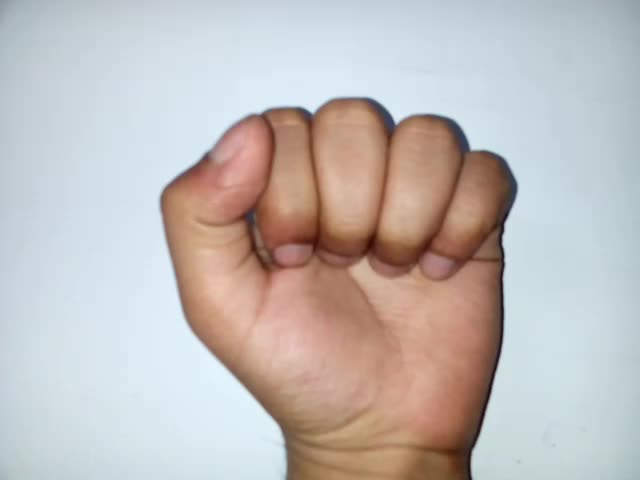
\includegraphics[width=.8\linewidth]{img/A}
		\caption{Orginalus paveikslėlis}
		\label{img:a-sign}
		%http://lifeprint.com/asl101/topics/wallpaper1.htm
	\end{minipage}\hspace{\fill}%
	\begin{minipage}{.3\textwidth}
		\centering
		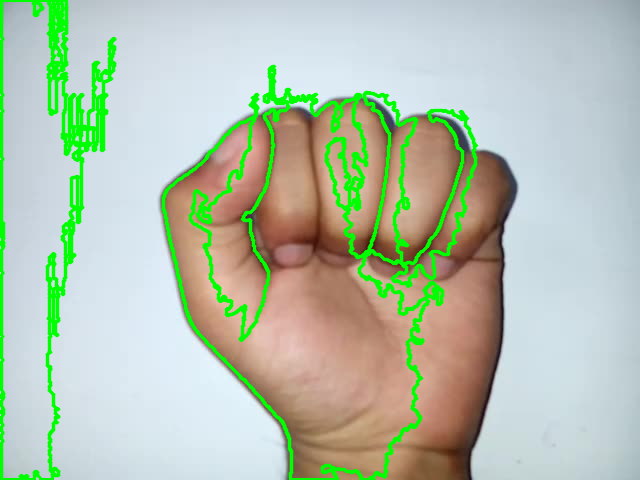
\includegraphics[width=.8\linewidth]{img/A-sobelX}
		\caption{Pritaikyta \textit{G\textsubscript{x}}}
		\label{img:a-sobelX}
		%https://www.kspvm.lm.lt/images/naujienos/2016-2017/kurciuju-filmuko-laimejimas/img/lt-gestu-abecele.jpg
	\end{minipage}\hspace{\fill}%
	\begin{minipage}{.3\textwidth}
		\centering
		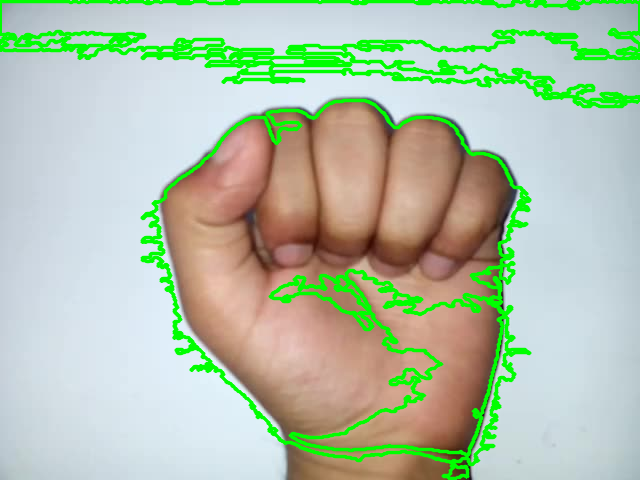
\includegraphics[width=.8\linewidth]{img/A-sobelY}
		\caption{Pritaikyta \textit{G\textsubscript{y}}}
		\label{img:a-sobelY}
		%https://www.kspvm.lm.lt/images/naujienos/2016-2017/kurciuju-filmuko-laimejimas/img/lt-gestu-abecele.jpg
	\end{minipage}\hspace{\fill}%
	\begin{minipage}{.3\textwidth}
		\centering
		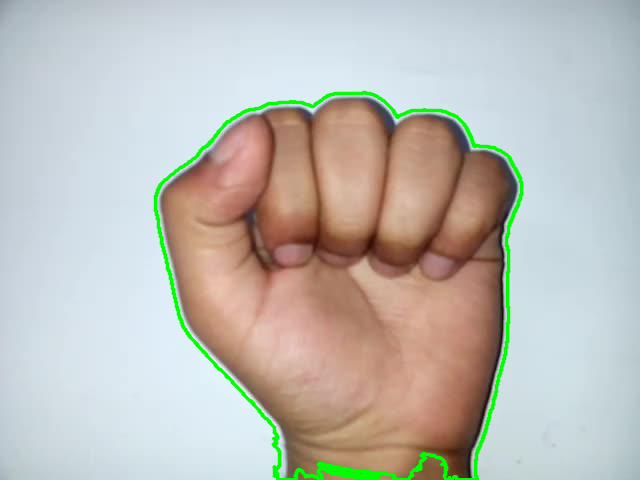
\includegraphics[width=.8\linewidth]{img/A-sobel}
		\caption{Pritaikyta \textit{G}}
		\label{img:a-sobel}
		%https://www.kspvm.lm.lt/images/naujienos/2016-2017/kurciuju-filmuko-laimejimas/img/lt-gestu-abecele.jpg
	\end{minipage}\hspace{\fill}%
	\begin{minipage}{.3\textwidth}
		\centering
		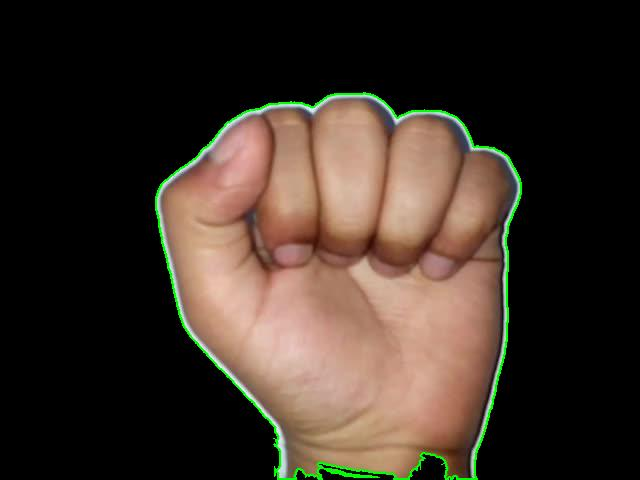
\includegraphics[width=.8\linewidth]{img/A-black}
		\caption{Be fono}
		\label{img:a-black-sign}
		%https://www.kspvm.lm.lt/images/naujienos/2016-2017/kurciuju-filmuko-laimejimas/img/lt-gestu-abecele.jpg
	\end{minipage}\hspace{\fill}%
	\begin{minipage}{.3\textwidth}
		\centering
		
\includegraphics[width=.8\linewidth]{img/A-white}
		\caption{Dviejų spalvų}
		\label{img:a-white-sign}
		%https://www.kspvm.lm.lt/images/naujienos/2016-2017/kurciuju-filmuko-laimejimas/img/lt-gestu-abecele.jpg
	\end{minipage}
\end{figure}

Prieš kadrui taikant Sobel funkcijas, reikia jį paruošti. Kadangi Sobel funkcijos ima matricas sudarytas iš \textit{3 $\times$ 3} skaičių, todėl reikia sušvelninti šalia esančius skaičius, tam jog jos rastų tikruosius kontūrus. Tą padaryti lengviausia uždedant kadrui, pavyzdžiui, 5\% miglą (\textit{angl. blur}). Uždėti miglą reikia tam, jog sumažėtų triukšmas (\textit{angl. noise}) kontūrams. 

Toliau, atiduodant kadrą Sobel funkcijoms, kadras yra konvertuojamas į skaičių į 3 masyvus, kurių kiekvienas atitinka po vieną RGB paletės spalvą, kur kiekvienas taškas turi savo skaičių – spalvos pasireiškimo ryškumo skaičių. Tuomet norint rasti visus kontūrus esančius kadre, taikome šiuos veiksmus:

\begin{enumerate}
	\item Einama per visus taškus esančius kadre ir taikoma \ref{eq:sobelgx} formulė, kur A - kiekvienas \textit{3 $\times$ 3} kadro taško spalvos mastyvas. Gaunamas \ref{img:a-sobelX} paveiksle pavaizduotas vaizdas;
	\item Einama per visus taškus esančius kadre ir taikoma \ref{eq:sobelgy} formulė, kur A - kiekvienas \textit{3 $\times$ 3} kadro taško spalvos mastyvas. Gaunamas \ref{img:a-sobelY} paveiksle pavaizduotas vaizdas;
	\item Apskaičiuojama dabartinio taško tikroji reiškė taikant \ref{eq:sobelg} formulę. Gaunamas \ref{img:a-sobel} paveiksle pavaizduotas vaizdas.
\end{enumerate}

Po šių žinsnių yra gaunama matrica taškų, kuriose keičiasi spalva. Dabar reikia išimti tuos taškus, kurie yra, \textit{pavyzdžiui}, ta pati balta spalva, tik kitokio atspalvio. Tam įgyvendinti lengviausia pasitelkus matricos vidurkį ir atmetus visus taškus, kurie yra mažesni už vidurkį. Kitaip tariant, išimant mažo skirtumo taškus. Po šių veiksmų lieka tik tie taškai, kurie jau turėtų priklausyti gesto kontūrui.

Ieškant kontūro taip pat reikėtų atmesti ir tuos kontūrus, kurie, \textit{pavyzdžiui}, neužima daugiau nei 5\% viso ploto ir tuomet nubrėžti kontūrą.

Kitas žingsnis – paversti kadrą į kompiuteriui suprantamą ir kuo paprastesnę kalbą. Turint kontūrus, galima kadrą paversti į dvispalvį kadrą, kur viskas, kas yra kontūre bus baltos spalvos, o viskas kas už kontūro ribų – juodos. Tam įgyvendinti reiktų pasidaryti kaukę (\textit{angl. mask}), kurioje viskas, kas už kontūro ribų bus, kaip ir minėta, juodos spalvos, tai kas šiuo atveju yra fonas (\textit{žr. \ref{img:a-black-sign} pav.}), o paskui ištrinti tai, kas yra kontūre ir padaryti baltos spalvos, tai kas šiuo atveju bus ženklas (\textit{žr. \ref{img:a-white-sign} pav.}).

Paskutinis žingsnis – prieš apmokant modelį reikia kadrą paversti duomenimis, iš kurių modelis galėtų būti apmokomas. Šioje vietoje buvo pasirinktas plačiausiai naudojamas metodas - kadrą paversti į skaičių matricą, kur balta spalva atitinka 255, o juoda - 0. Ši konvertacija pasirinkta pagal spalvų kodus. Jau pavertus kadrą į skaičių matricą, ši buvo suplokštinta, kad būtų gaunama vienmatė matrica. Ir galiausiai į vieną bendrą duomenų rinkmeną (\textit{angl. file}) surašomi duomenys tokia seka: pirmas eilutės langelis - gestą atitinkanti abėcėlės raidė, o visi likę šios eilutės langeliai užpildomi vienmatės kadro matricos duomenis skaičių pavidalu, apie kuriuos buvo kalbėta šios pastraipos pradžioje.

\subsubsection{Apsimokančių sistemų apmokymas iš Sobel branduoliu apdoroto kadro}
Turint rinkmeną, kurioje yra surašyti visi apmokymams skirtų kadrų duomenys, bus aptariama, kaip iš šių duomenų apmokyti sistemą.

Šiame poskyryje bus aptarta keletą objektams atpažinti populiarių technikų, kuriomis remiantis galima apmokyti sistemą atpažinti gestus.

\begin{equation}\label{eq:z}
	z = \theta_0+\theta_1x_1+\theta_2x_2+\theta_3x_1^2+\theta_4x_1x_2+...
\end{equation}

\ref{eq:z} formulė apibrėžia, kaip bus apskaičiuojamas parametras \textit{z}, kai norima susidaryti pasirinktos formos plotą, pagal kurį gestas priklausys arba nepriklausys išmoktai abėcėlės raidei. \textit{x\textsubscript{1}} ir \textit{x\textsubscript{2}} yra koordinačių ašys, kuriose yra išsidėstę taškai.

\subsubsubsection{Logistinės regresijos algoritmas}

\textbf{Logistinės regresijos algoritmas} dar žinoma kaip „logistic regression“ algoritmas. Tai – vienas populiariausių šiuo metu naudojamų klasifikavimo algoritmų.

\begin{equation}\label{eq:lr1}
	0 \leq h_\theta^i(x) \leq 1; i = 1, 2, ..., 24
\end{equation}

Remiantis \ref{eq:lr1} formule, apsibrėžiama, jog tikimybės kiekvienai raidei bus ne mažesnės nei 0 ir ne didesnės nei 1, o \textit{i} pasako kelinta raidė tyrinėjama, kur, tarkime, A = 1, B = 2, ir t.t.


\begin{equation}\label{eq:lr2}
	h_\theta^i(x) = P(y=i | x; \theta)
\end{equation}

Remiantis \ref{eq:lr2} formule, apsibrėžiama tikimybės formulė, kuriai kaip parametras paduodamas gesto numeris (tarkime, kad raidė A = 1, B = 2 ir t.t.), bei bus naudojamasi parametrais $\theta$, kur  $\theta$ - svorių vertės, kuriomis remiantis apskaičiuojama tikimybė 
\textit{P}. $\theta$ reikšmes apmokomos sistemos apsiskaičiuoja pačios skirtingais algoritmais, todėl šiame darbe jie nagrinėjami nebus.

\begin{equation}\label{eq:lr3}
	h_\theta(x)= g(z)
\end{equation}


Remiantis \ref{eq:lr3} formule, galima apsibrėžti ne tik tiesės atskyrimą (pagal įprastinę šios formulės reikšmę), bet ir įvairias formas, kaip šiuo nagrinėjamu atveju, tarkime, delno formą. 

\begin{equation}\label{eq:lr4}
	h_\theta(x) = \frac{1}{1+e^{-z}}
\end{equation}

Galiausiai, \ref{eq:lr4} formulėje galime matyti, jog tikimybė yra apskaičiuojama remiantis \ref{eq:lr3} formulėje apsibrėžtos formos pavidalu.

\subsubsubsection{Linijinis palaikančiųjų vektorių algoritmas}

\textbf{Linijinis palaikančiųjų vektorių algoritmas} dar žinomas kaip „Linear Support Vector Machine“ algoritmas.

Iš esamų duomenų aibės taškų, šiuo atveju – skirtingų gestų raidžių taškų, yra sudaroma matrica, kurioje tarp skirtingų gestų yra nubrėžiamas vektorius, kuris nusako, kurioje vietoje bus traktuojamas vienas gestas, kurioje - kitas. Iki vektoriaus yra parenkamas didžiausias galimas atstumas nuo artimiausių prie vektoriaus esančių duomenų taškų. 

Pats principas $\theta$ parinkimui yra labai panašus kaip loginėje regresijoje, bei \textit{z} yra paskaičiuojama pagal tą pačią formulę.

Šis metodas yra geresnis, kai yra ganėtinai didelis skirtumas tarp duomenų aibės taškų ir lengvai nubrėžiami vektoriai, nes nesikerta duomenų aibės. Dar vienas šio metodo privalumas yra tas, jog nubrėžus vektorių esant didžiausiam atstumui tarp duomenų taškų, esančių arčiausiai vektoriaus, ganėtinai nesunkiai yra nustatoma, kuriai pusei (šiuo atveju gestui), priklauso duotasis taškas.

Tačiau iš kitos pusės, šis metodas nėra ypač lengvai apdorojantis duomenis, jei duomenų aibės yra persidengiančios, todėl gestų kalbos atpažinimo atveju šis metodas nėra labai tikslus, nes gestų duomenų aibės yra persidengiančios didžiaja dalimi ir skiriasi tik pirštų padėtys.

\subsubsubsection{K artimiausių kaimynų algoritmas}

\textbf{K artimiausių kaimynų algoritmas} dar žinomas kaip „k-nearest neighbors“ algoritmas.

Viskas yra suskirstoma į aibes ir pagal tašką ieškomas artimiausias kaimynas arba kaimynų aibė ir, priklausomai nuo to, kurių kaimynų daugiausia, parenkama reikšmė, kokia bus naujojo taško reikšmė.

Šis algoritmas kaip ir prieš tai aptartas linijinis palaikančiųjų vektorių algoritmas nėra idealus pasirinkimas gestų kalbos atpažinimui, nes, tarkime, jei būtų imamas delno vidurio taškas galimi visi 24 variantai ir tik kampuose, žiūrint į atlenktų pirštų skaičių būtų galima nuspręsti, kuris gestas rodomas.


\subsection{Sistemos apmokymas, naudojantis konvoliucinio neuroninio tinklo modeliu}

Prieš apmokant sistemą, naudojantis konvoliucinio neuroninio tinklo modeliu, pirma bus aptariama, kas yra konvoliucinis bei telkimo sluoksniai, o vėliau - kaip apmokyti sistemą.

\subsubsection{Konvoliucinis sluoksnis}

Konvoliucinis sluoksnis turi tokius parametrus:
\begin{itemize}
	\item Priima matricą, sudarytą iš \textit{\textbf{W\textsubscript{1} $\times$ H\textsubscript{1} $\times$ D\textsubscript{1}}}, kur \textit{\textbf{W\textsubscript{1}}} - plotis, \textit{\textbf{H\textsubscript{1}}} - aukštis ir \textit{\textbf{D\textsubscript{1}}} - gylis;
	\item Reikalingi papildomi parametrai:
		\begin{itemize}
			\item Filtrų skaičius \textbf{\textit{K}} (dažniausiai naudojamas 2-to laispnis);
			\item Filtro dydis \textbf{\textit{F}} (dažniausiai naudojama - 3, todėl filtro matrica būna - 3 $\times$ 3 filtrai);
			\item Žingsnis, per kiek paslenkamas filtras \textbf{\textit{S}};
			\item Papildomas rėmelis duotajai matricai, sudarytas iš 0, \textbf{\textit{P}};
		\end{itemize}
	\item Sudaroma matrica \textit{\textbf{W\textsubscript{2} $\times$ H\textsubscript{2} $\times$ D\textsubscript{2}}}, kur \textit{\textbf{W\textsubscript{2}}} - plotis, \textit{\textbf{H\textsubscript{2}}} - aukštis ir \textit{\textbf{D\textsubscript{2}}} - gylis, kur:
		\begin{itemize}
			\item \textit{\textbf{W\textsubscript{2} = (W\textsubscript{1} – F + 2P)/S + 1}};
			\item \textit{\textbf{H\textsubscript{2} = (H\textsubscript{1} – F + 2P)/S + 1}};
			\item \textit{\textbf{D\textsubscript{2} = K}}.
		\end{itemize}
\end{itemize}

Sluoksnis, kuris pagal filtrą nusprendžia, kokia išeities matricą bus gaunama. Tarkime, jog bus imamas filtras, kuris yra \textit{3 $\times$ 3} matrica. Kadrą, kaip jau buvo minėta, galima išskirstyti į tris skirtingus sluoksnius - raudonos, žalio ir mėlynos spalvos. Pavertus šiuos sluoksnius skaičių matricomis, kur 0 – spalva nenaudojama, o 255 – spalva naudojama pilnai ryškiai, gaunamos matricos, kurios nusako, kaip kiekviename taške ryškiai yra naudojama tam tikra spalva.

Kaip pavyzdį galima panagrinėti \textit{7 $\times$ 7} kadro matricą su \textbf{\textit{F}} = 3, \textbf{\textit{S}} = 1, \textbf{\textit{P}} = 1, \textbf{\textit{K}} = 1. Einant taškas po taško per kadro kiekvienos spalvos matricą, imamos \textit{3 $\times$ 3} matricos, kurios yra sudauginamos su filtro matricomis. Taip gaunama matrica, kuria remantis bus galima išskirti savybes.

\textit{Pavyzdys:}

\begin{equation}\label{eq:convl}
	\begin{bmatrix}
	1 & 1 & 0 & 1 & 0 & 1 & 0 \\
	1 & 0 & 1 & 1 & 1 & 0 & 1 \\
	1 & 1 & 0 & 1 & 1 & 0 & 1 \\
	1 & 1 & 0 & 1 & 0 & 1 & 0 \\
	1 & 0 & 1 & 1 & 1 & 0 & 1 \\
	1 & 1 & 0 & 1 & 1 & 0 & 1 \\
	1 & 1 & 0 & 1 & 0 & 1 & 0
	\end{bmatrix}
	*
	\begin{bmatrix}
	1 & 0 & 1 \\
	0 & 1 & 0 \\
	1 & 0 & 1
	\end{bmatrix}
	=
	\begin{bmatrix}
	\colorbox{green}{1} & \colorbox{pink}{3} & 1 & 3 & 1 & 3 & 0 \\
	3 & 2 & 5 & 2 & 4 & 2 & 2 \\
	2 & 4 & 3 & 3 & 3 & 2 & 2 \\
	2 & 4 & 3 & 4 & 2 & 5 & 0 \\
	3 & 2 & 5 & 2 & 4 & 2 & 2 \\
	2 & 4 & 3 & 3 & 3 & 2 & 2 \\
	3 & 2 & 2 & 2 & 1 & 3 & 0
	\end{bmatrix}
\end{equation}

\begin{equation}\label{eq:convl1}
	0*1+0*0+0*1+0*0+1*1+1*0+0*1+1*0+0*1=\colorbox{green}{1}
\end{equation}


\begin{equation}\label{eq:convl2}
	0*1+0*0+0*1+1*0+1*1+0*0+1*1+0*0+1*1=\colorbox{pink}{3}
\end{equation}

\ref{eq:convl} formulėje yra pateikta \textit{7 $\times$ 7} matrica sudauginta su \textit{3 $\times$ 3} filtru. Panagrinėsime pirmos eilutės pirmąjį (\textit{žr. \ref{eq:convl1} formulę}) ir antrąjį (\textit{žr. \ref{eq:convl2} formulę}) narius. Pirmasis narys yra kampinis skaičius 1. Todėl jis dauginamas su filtro viduriniuoju nariu. Kadangi dabar filtras „išlenda“ iš matricos rėmų, tai įsivaizduojama, kad yra kadro matricai rėmelis, kuris yra sudarytas iš 0 (rėmelis \textit{P}). \ref{eq:convl1} ir \ref{eq:convl2} formulėse pirmasis sandaugos narys - \textit{7 $\times$ 7} kadro matricos narys, antrasis - \textit{3 $\times$ 3} filtro matricos narys.

\begin{equation}\label{eq:nuliai}
M=\frac{F-1}{2}
\end{equation}

\ref{eq:nuliai} formulėje yra pateikta, kokio dydžio papildomą išorinį sluoksnį (rėmelį \textit{P}) sudarytą iš 0 konvoliuciniai neuroniniai tinklai dažniausiai naudoja. Čia \textit{M} yra sluoksnio plotis pridedamas prie kiekvienos matricos kraštinės, o \textit{F} – filtro matricos dydis. Tai naudojama tam, kad būtų gaunama tokio pačio dydžio matrica, kokia buvo paduota filtrui apdoroti.


\subsubsection{Telkimo sluoksnis}

Telkimo sluoksnis turi tokius parametrus:
\begin{itemize}
	\item Priima matricą, sudarytą iš \textit{\textbf{W\textsubscript{1} $\times$ H\textsubscript{1} $\times$ D\textsubscript{1}}}, kur \textit{\textbf{W\textsubscript{1}}} - plotis, \textit{\textbf{H\textsubscript{1}}} - aukštis ir \textit{\textbf{D\textsubscript{1}}} - gylis;
	\item Reikalingi papildomi parametrai:
	\begin{itemize}
		\item Filtro dydis \textbf{\textit{F}} (dažniausiai naudojama - 2, todėl fitro matrica - 2 $\times$ 2);
		\item Žingsnis, per kiek paslenkamas filtras \textbf{\textit{S}} (dažniausiai naudojams žingsnis - 2);
	\end{itemize}
	\item Sudaroma matrica \textit{\textbf{W\textsubscript{2} $\times$ H\textsubscript{2} $\times$ D\textsubscript{2}}}, kur \textit{\textbf{W\textsubscript{2}}} - plotis, \textit{\textbf{H\textsubscript{2}}} - aukštis ir \textit{\textbf{D\textsubscript{2}}} - gylis, kur:
	\begin{itemize}
		\item \textit{\textbf{W\textsubscript{2} = (W\textsubscript{1} – F)/S + 1}};
		\item \textit{\textbf{H\textsubscript{2} = (H\textsubscript{1} – F)/S + 1}};
		\item \textit{\textbf{D\textsubscript{2} = D\textsubscript{1}}}.
	\end{itemize}
\end{itemize}


Kaip buvo minėta anksčiau, telkimo sluoksnis yra skirtas sumažinti matricą arba kitais žodžiais tariant - kadrą. Telkimo sluoksnis dažniausiai taiko arba vidutinės arba didžiausios reikšmės atrinkimo algoritmą. Imkime kaip pavyzdį, kad \textbf{\textit{S}} = 3, \textbf{\textit{F}} = 3. Bus taikomas maksimalaus telkimo principas, kuris nusako, jog paėmus matricos poaibį yra išrenkama didžiausia reikšmė.

\textit{Pavyzdys:}
\begin{equation}\label{eq:poll}
	\begin{bmatrix}
	1 & 3 & 1 & 3 & 1 & 3 \\
	3 & 2 & 5 & 2 & 4 & 2 \\
	2 & 4 & 3 & 3 & 3 & 2 \\
	2 & 4 & 3 & 4 & 2 & 5 \\
	3 & 2 & 5 & 2 & 4 & 2 \\
	2 & 4 & 3 & 3 & 3 & 2
	\end{bmatrix}
	= 
	\begin{bmatrix}
	\colorbox{green}{5} & \colorbox{pink}{4} \\
	5 & 5 
	\end{bmatrix}
\end{equation}
\begin{equation}\label{eq:poll1}
	max(
	\begin{bmatrix}
	1 & 3 & 1 \\
	3 & 2 & 5 \\
	2 & 4 & 3
	\end{bmatrix}
	) = \colorbox{green}{5}
	%1, 3, 1, 3, 2, 5, 2, 4, 3
\end{equation}
\begin{equation}\label{eq:poll2}
	max(
	\begin{bmatrix}
	3 & 1 & 3 \\
	2 & 4 & 2 \\
	3 & 3 & 2
	\end{bmatrix}
	) = \colorbox{pink}{4}
\end{equation}
\ref{eq:poll} formulėje parodyta, kaip pritaikius \textit{3 $\times$ 3} telkimo filtrą gaunama beveik 90\% mažesnė matrica. Mažinimas vyksta taip: imama filtro dydžio matrica, pradėdedant nuo kairiojo viršutinio kampo. Tuomet iš tos matricos išrenkama didžiausia reikšmė (\textit{žr. \ref{eq:poll1} formulę}) ir į naująją matricą ji įrašoma. Tuomet, kadangi jau iš pirmosios \textit{3 $\times$ 3} matricos yra išrinkta didžiausia reikšmė (jei būtų taikomas vidutinės reikšmės atrinkimo algoritmas, būtų imama šios matricos vidutinė reikšmė), imama kitą į dešinę esanti matrica, kuri nepersidengia su pirmąja, nes \textbf{\textit{S}} = 3,  ir iš jos taip pat išrenkama didžiausia reikšmė (\textit{žr. \ref{eq:poll2} formulę}). Taip filtras yra pritaikomas ir likusioms matricos dalims. Jei filtras „užeina“ už kadro matricos ribų, interpretuojama, jog tose vietose yra 0.

\subsubsection{Apmokymas naudojantis konvoliucinio neuroninio tinklo modeliu}

Kiekvieną sistemą galima apmokyti naudojantis kovoliuciniu neuroniniu tinklo modeliu arba nuodugniai (kuomet apmokomas modelis neturi jokių duomenų), arba dalinai (kuomet pasinaudojama jau veikiančiu modeliu ir nutrinamas paskutinis ar keli paskutiniai sluoksniai). Apmokymas nuo pat pradžių dažniausiai reikalauja labai daug laiko resursų, nes užtrunka labai daug laiko. Šis modelis retai naudojamas praktikoje. Dažniausiai naudojamas dalinis apmokymas, pasinaudojus jau sukurtu modeliu galima jį pakartotinai apmokyti norimam rezultatui gauti. 

Bene vienas lengviausiai naujokui suprantamų modelių yra VGG16 architektūros modelis. Tai 16 sluoksnių modelis, kurio architektūra pateikta 1 priede. Tai penkių žingsnių modelis, kuris taiko konvoliucijos ir telkimo sluoksnius kiekviename žingsnyje. \textit{Pavyzdžiui}, pirmame žingsnyje iš kadro yra 64 sugeneruojami nauji kadrai, kuriems pritaikomi 64 skirtingi filtrai (\textit{žr. \ref{img:filtersvgg} pav.}). Taikoma du kartus konvoliucija ir tuomet vieną kartą telkimas. Po visų penkių žingsnių, gaunamas pilnai apjungtas sluoksnis, kuris jau geba atpažinti objektus. 

\begin{figure}[H]
	\centering
	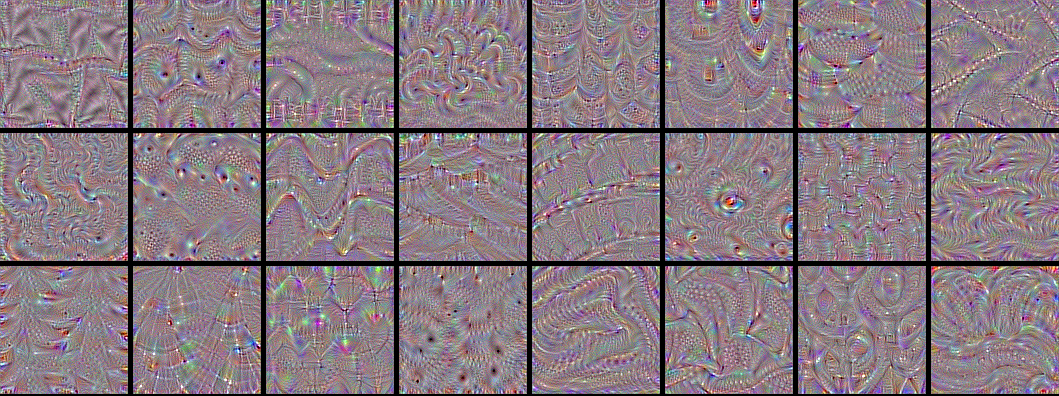
\includegraphics[width=.6\linewidth]{img/vgg16filters}
	\caption[]{Filtrų pavyzdžiai\footnotemark}
	\label{img:filtersvgg}
\end{figure}
\footnotetext{\url{https://blog.keras.io/how-convolutional-neural-networks-see-the-world.html}}

\section{Praktinis gestų kalbos apmokyto modelio pritaikymas}

Praeituose skyriuose buvo aptarta, kokie būdai yra galimi apmokyti sistemą atpažinti gestų kalbą. Šiame skyriuje bus aprašyta, kaip šie aprašyti žingsniai buvo pritaikyti praktiškai.

\subsection{Duomenys}
Duomenys (programinis kodas ir kadrai) buvo parsisiųsti iš jau įgyvendintų pavyzdinių gestų kalbos sistemų. Viename iš duomenų rinkinių buvo po 150-250 gesto kadrų kiekvienai raidei (pavyzdys pateiktas \ref{img:a-sign} paveikslėlyje). Taip pat pasinaudojus šių kadrų paprastumu dėl šviesaus ir vienspalvio fono, buvo uždėti skirtingi fonai.

\begin{figure}[H]
	\begin{minipage}{.5\textwidth}
		\centering
		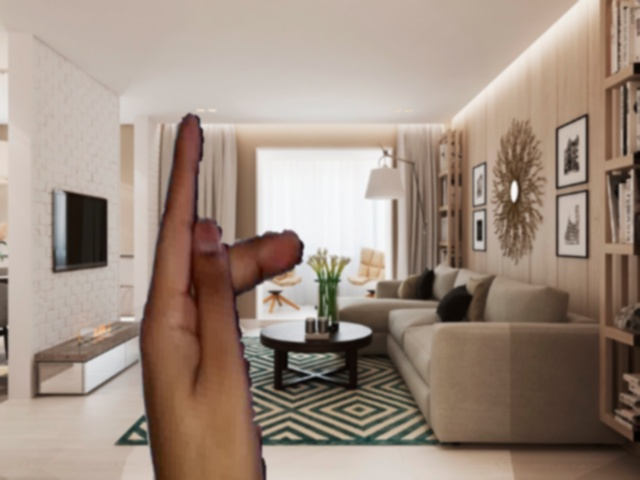
\includegraphics[width=.8\linewidth]{img/K1}
		\caption{K raidės gestas su pakeistu fonu}
		\label{img:a-sign-first}
		%http://lifeprint.com/asl101/topics/wallpaper1.htm
	\end{minipage}\hspace{\fill}%
	\begin{minipage}{.5\textwidth}
		\centering
		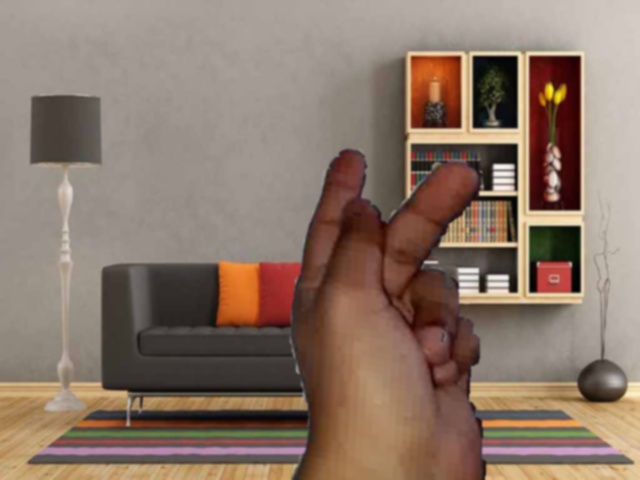
\includegraphics[width=.8\linewidth]{img/K2}
		\caption{K raidės gestas su pakeistu fonu}
		\label{img:a-sign-second}
		%https://www.kspvm.lm.lt/images/naujienos/2016-2017/kurciuju-filmuko-laimejimas/img/lt-gestu-abecele.jpg
	\end{minipage}\hspace{\fill}%
\end{figure}

Kiekvienam iš 150-250 kadrų kiekvienai raidei buvo uždėta po du atsitiktinai sugeneruotus fonus. Todėl buvo sudaryta po 400 gesto kadrų kiekvienai raidei, pakeičiant jų vietą, kampą, ištempimą ir kt.

\subsection{Duomenų suskirstymas}

Duomenys buvo suskirstyti į aplankus, kur aplanko pavadinimas rodo raidę, kurią atitinka gestas. Taip buvo sukurti 24 aplankai kiekvienai iš 24 ASL raidžių. Visi duomenys buvo suskirstyti į tris aplankus, kurie buvo skirti apmokymui, patikrinimui (ne visais atvejais buvo naudojamas) ir testavimui. Duomenų imta labai nedaug - apmokymui skirtų gestų kadrų buvo po 400 kiekvienai raidei (vėliau kito), patikrinimui - 100 kiekvienai raidei ir dar 240 testavimui skirtų kadrų.

\subsection{Sistemos apmokymas}
Tyrimas buvo atliktas keliais skirtingais būdais.

\subsubsection{Sistemos apmokymas naudojant įprastus metodus}
Sistema buvo apmokyta naudojantis OpenCV atviro kodo biblioteka. Pasinaudota Sobel branduoliu ir logistinės regresijos bei linijiniu palaikančiųjų vektorių algoritmais. Reikėtų paminėti, jog šioje vietoje buvo pasirinkti kadrai, kurie yra su šviesiu fonu ir lengvai atskiriamas gestas nuo fono. Tuomet gestų duomenys pasinaudojus \textit{sklearn} apmokomos sistemos pagalba buvo sudėti į rinkmeną, kuri vėliau pasinaudojus šiais duomenimis atskirtų, koks gestas yra rodomas. Po apmokymų, atpažinimas svyravo tarp 95-98\%, jei turime lengvai nuimamą foną. Tačiau, jei fonas būdavo įvairus ir skirdavosi apšvietimas, sistema gestų arba neatpažindavo, arba atpažindavo neteisingai, o tikslumas po apmokymo svyravo tarp 50-60\%, todėl galima apibendrintai pasakyti, jog šių metodų tikslumas priklauso nuo duomenų kiekio ir programinio kodo, kuris gerai sugebėtų nuimti triukšmą ir esantį foną, kad liktų tik švarus gesto kontūras. Sistemos apmokymas truko apie 5 valandas, turint 400 kadrų kiekvienai ASL abėcėlės raidei.

\textbf{Šių metodų minusai}:
\begin{enumerate}
	\item Sunku atskirti foną nuo gesto
	\item Reikia daug skirtingų duomenų, kad algoritmai ganėtinai tiksliai atskirtų gestus
	\item Sunkiai panaudojama prie bet kokio apšvietimo ir fono
\end{enumerate}

\subsubsection{Sistemos apmokymas naudojant konvoliucinio neuroninio tinklo modelį}

Buvo pasirinkta sistemą naudojant konvoliucinio neuroninio tinklo modelį keliais skirtingais būdais:
\begin{enumerate}
	\item Nuodugiai
	\item Dalinai
\end{enumerate}
Šiame apmokyme buvo pasinaudota gestais, kurie buvo modifikuoti pakeičiant foną, poziciją, pasukimo kampą, ištempimą ir kt.


\subsubsubsection{Nuodugnus apmokymas}
Nuodugniam apmokymui buvo pasirinkta pasinaudoti „Keras“ giliojo mokymosi biblioteka pasinaudojant „Theano“. Taip pat buvo pasirinkta VGG16 architektūra - 16 sluoksnių apmokymo modelis, kurio architektūros modelis pateiktas 1 priede (\textit{žr. \ref{img:vgg} pav.}). Apmokant sistemą nuodugniai buvo pasirinkta išbandyti apmokyti atpažinti tik dvi ASL raides - A ir B. Sistemos apmokymas truko kiek daugiau nei 2,5 valandos, turint 400 kiekvieno gesto kadrų mokymui ir 200 pasitikrinimui. Po šių apmokymų atpažinimas svyravo tarp 50-60\%. Tačiau išbandžius sistemą, buvo atpažįstami gestai esant bet kokiam apšvietimui, atstumui ir kt. Bendras tikslumas buvo geresnis nei naudojantis įprastais metodais.

\textbf{Trūkumai}:
\begin{enumerate}
	\item Reikia daug duomenų, kad sistema gerai apsimokytų;
	\item Užtrunka daug laiko.
\end{enumerate}

\subsubsubsection{Dalinis apmokymas}
Daliniam apmokymui buvo pasinaudota „Inception-v3“ jau apmokytu modeliu, kuris yra „TensorFlow“ bibliotekoje. Buvo nutrinamas paskutinis sluoksnis ir sistema papildomai apmokyta atpažinti tik ASL abėcėlės raides. 
\textbf{Pirmasis bandymas}

Pirmasis apmokymas buvo skirtas atpažinti tik dvi raides - A ir B. Kiekvienai raidei buvo skirta po 400 kadrų. Po apmokymo, kuris užtruko apie 5 minutes, atpažinimas svyravo tarp 95-98\%, tačiau testuojant, visi atsakymai buvo teisingi.

\textbf{Antrasis bandymas}

Antrasis apmokymas buvo skirtas atpažinti visas ASL abėcėlės 24 statines raides. Sistemos apmokymas užtruko apie 30 minučių.

Su 400 kadrų kiekvienai ASL abėcėlės raidei, \ref{img:acc} grafikas rodo apmokyto modelio tikslumą. Gesto atpažinimo tikslumas su 400 kadrų yra apie 60\%, kiek mažesnis tikslumas yra patikrinimo, bet taip pat apie 60\%. Grafike oranžinė linija rodo apmokymo tikslumą, o mėlyna - patikrinimo. Šis apmokymas buvo atliktas su 500 apmokymo žingsnių.

\begin{figure}[H]
	\centering
	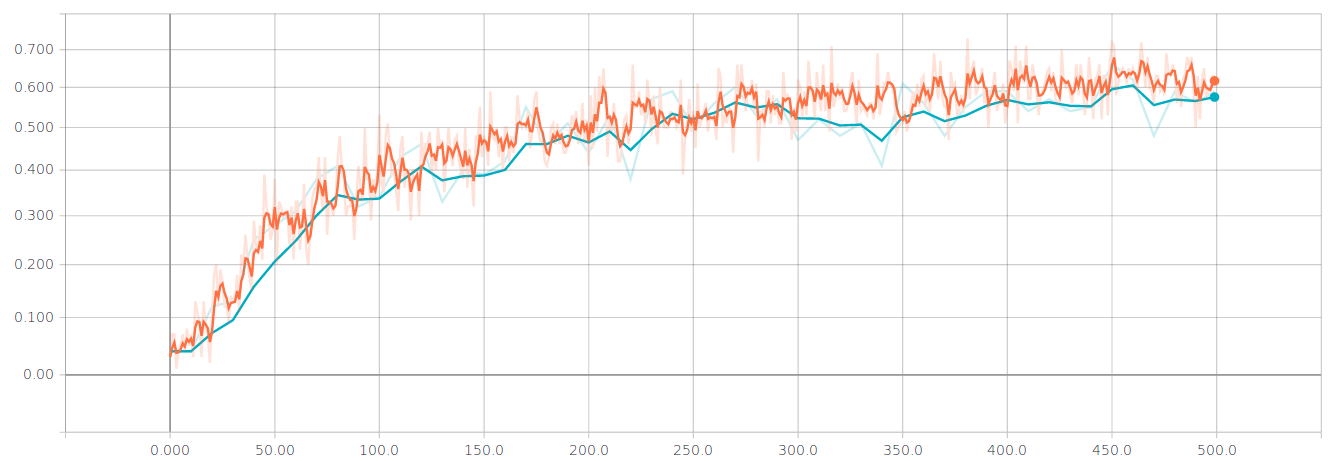
\includegraphics[width=.8\linewidth]{img/accuracy}
	\caption{Tikslumo grafikas su 400 kadrų ir 500 apmokymo žingsnių}
	\label{img:acc}
\end{figure}


\textbf{Trečiasis bandymas}

Pasirinkti tie patys duomenys – 400 kadrų kiekvienai ASL abėcėlės raidei, tik padidintas apmokymo žingsnių skaičius iki 5000.

\begin{figure}[H]
	\centering
	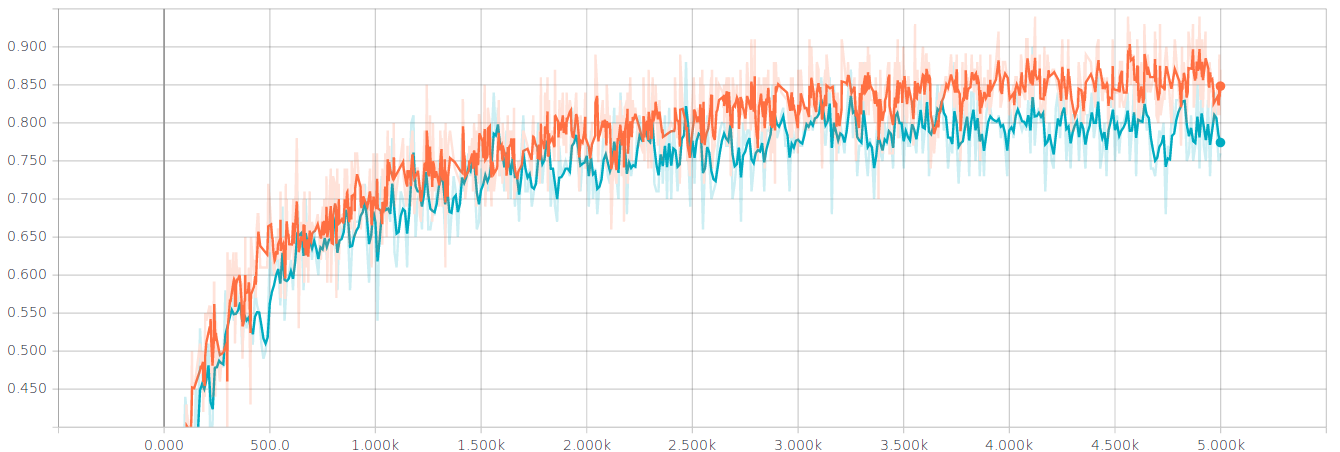
\includegraphics[width=.8\linewidth]{img/accuracy2}
	\caption{Tikslumo grafikas su 400 kadrų ir 5000 apmokymo žingsnių}
	\label{img:acc2}
\end{figure}

Su 400 kadrų kiekvienai ASL abėcėlės raidei, \ref{img:acc2} grafikas rodo apmokyto modelio tikslumą. Šiuo atveju, kaip ir buvo minėta, žingsnių skaičius pasirinktas 5000. Sistemos tikslumas padidėjo nuo 60\% iki beveik 85\% mokymosi metu ir 77\% patikrinimo metu. Rezultatai kur kas gersni nei antruoju bandymu, tačiau testuojant rezultatai prastesni, nes to kaip priežastis galėtų būti daugiau skirtingų klasių.

\textbf{Ketvirtasis bandymas}

Ketvirtasis apmokymas buvo skirtas taip pat atpažinti visas ASL abėcėlės raides, tačiau buvo naudojama po 1000 kadrų kiekvienai raidei ir duomenys papildyti gestą horizontaliai apverčiant prie tų duomenų, kurie buvo. Sistema buvo apmokyta per 45 minutes ir pasirinkta naudoti 5000 apmokymo žingsnių. Mokymosi tiksumas – 85\%, o patikrinimo tikslumas – 79\% (\textit{žr. \ref{img:acc3} pav.}). Kadangi kadrai buvo labai panašūs į prieš tai buvusius 400, tik padidintas jų skaičius, tai ir rezultatai beveik nesiskiria nuo praeito bandymo.

\begin{figure}[H]
	\centering
	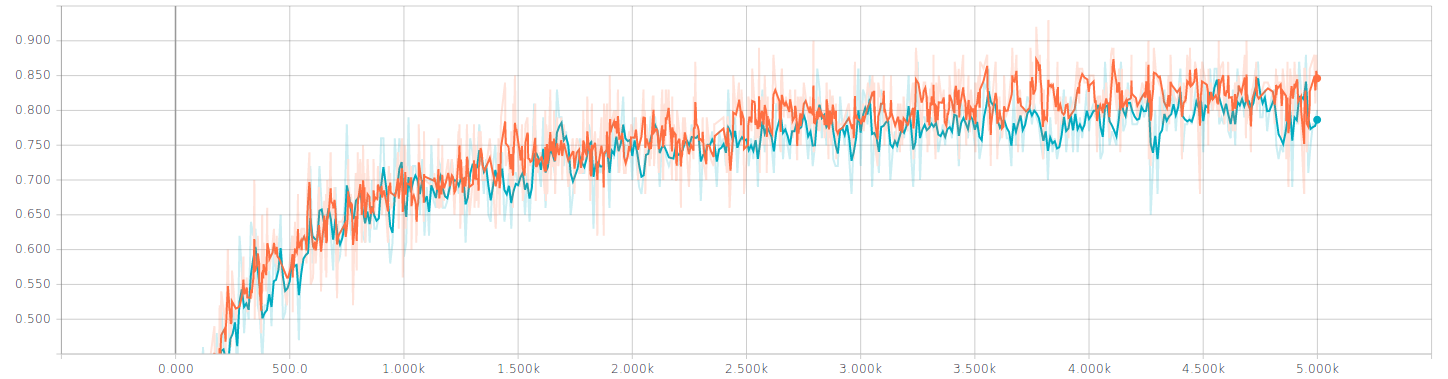
\includegraphics[width=.8\linewidth]{img/accuracy3}
	\caption{Tikslumo grafikas su 1000 kadrų ir 5000 apmokymo žingsnių}
	\label{img:acc3}
\end{figure}

Šio bandymo metu buvo padaryta 240 kadrų - po 10 kadrų kiekvienai abėcėlės raidei. Šie kadrai nebuvo skirti nei apmokymui, nei patikrinimui. Su visiškai nauja ir sistemai nematyta aibe buvo atliktas testavimas. Gautas 15,13\% tikslumas su šiais kadrais, kuomet sistema tiksliai atpažįsta gestą. 25,21\% tikslumas, kai tikrasis gestas yra pirmasis arba antrasis sistemos pasirinkimas. Ir galiausiai 38,24\% jei tikrasis atsakymas yra tarp pirmų penkių sistemos spėjimų.

\textbf{Penktasis bandymas}

Penktuoju bandymu buvo naudojama dar daugiau duomenų. Panaudota apie 3000 kadrų kiekvienai abėcėlės raidei, pasirinktas 5000 apmokymo žingsnių metodas. Duomenys naudoti iš trijų skirtingų duomenų rinkinių. Šiu atveju mokymosi tikslumas nukrito iki 80\% ir išaugo iki 80\% pasitikrinimo metu (\textit{žr. \ref{img:acc4} pav.}). Galima pastebėti, jog bendras mokymosi tikslumas nelabai pakito, tačiau padidėjo patikrinimo tikslumas.

\begin{figure}[H]
	\centering
	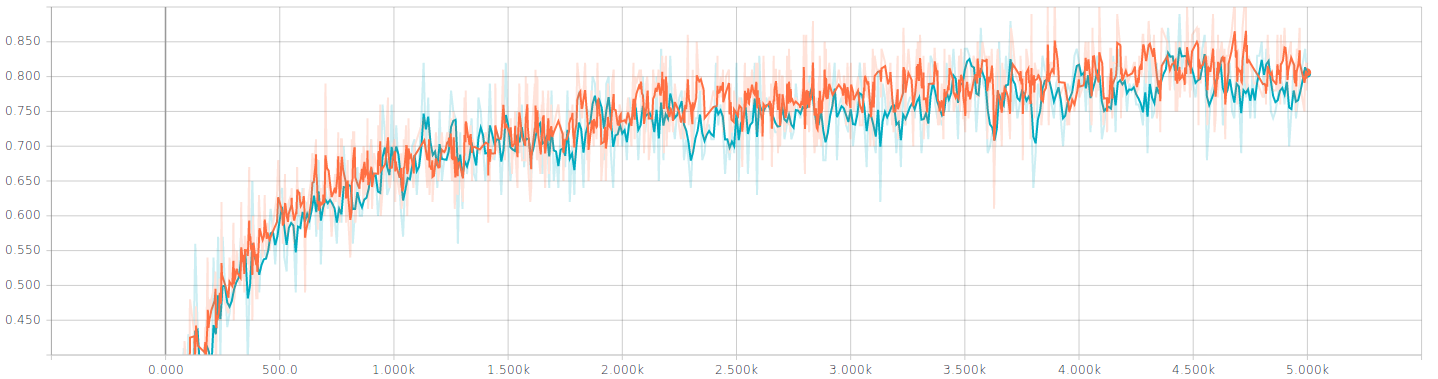
\includegraphics[width=.8\linewidth]{img/accuracy4}
	\caption{Tikslumo grafikas su 3000 kadrų ir 5000 apmokymo žingsnių}
	\label{img:acc4}
\end{figure}

Kaip ir ketvirtuoju bandymu sistema buvo ištestuota. Gauti rezultatai: 14,71\% pirmasis pasirinkimas, 20,17\% - vienas iš dviejų pirmųjų ir 34,45\% jei teisingas atsakymas yra tarp pirmų 5 sistemos bandymų atspėti raidę.

\subsection{Apibendrinimas}
Buvo išbandyti trys skirtingi apmokymų būdai. Geriausias ir tiksliausiai atpažįstantis būdas gautas, naudojant konvoliucinio neuroninio tinklo dalinio apmokymo modelį, kuris nesunkiai esant įvairiems apšvietimams ir gestų rodymo kampams atpažįsta gestus, net ir esant nedidelei duomenų aibei. Tačiau esant kuo didesnei duomenų aibei, dideliam apmokymo žingsnių skaičiui, sistemos atpažinimas tapo iškart žymiai geresnis. Norint dar tikslesnių duomenų, reiktų sistemą apmokyti turint daugiau duomenų, daryti dar didesnę duomenų augmentaciją, pasinaudoti skirtingais duomenų rinkiniais. Pastebėta, jog padidinus apmokymo žingsnių skaičių duomenų atpažinimo rodikliai pakilo, tačiau didinant apmokomų duomenų kiekį rezultatai nelabai skiriasi. Bendrus rezultatus galima palygtinti \ref{tab:title} lentelėje. Reiktų paminėti ir tai, jog testuojant sistemą rezultatai buvo ganėtinai prasti. Pastebėta, kad ketvirtojo bandymo apmokymo tikslumas atsispindi ir testavimo statistikoje - ketvirtuoju bandymu apmokyta sistema yra tikslesnė (\textit{žr. \ref{tab:title2} pav.}). Taip galėtų būti dėl kelių priežasčių. Viena iš šių priežasčių - skirtingose duomenų aibėse galimai yra įsipainioję netikslūs duomenys, nes papildomai duomenų aibės nebuvo perrenkamos ir peržiūrimos jas išvalant.

   
   
\vspace{\baselineskip}
\begin{minipage}{\linewidth}
	\centering
	\captionof{table}{Konvuliacinių neuroninių tinklų ASL abėcėlės apmokymų statistika} \label{tab:title} 
	\begin{tabular}{ |c|c|c|c|c| } 
		\hline
		 & \thead{Antras\\bandymas} & \thead{Trečias\\bandymas} & \thead{Ketvirtas\\bandymas} & \thead{Penktas\\bandymas} \\
		\hline
		%\multirow {Multiple row} & cell2 & cell3 \\ 
		Apmokymo tikslumas & 60\% & 85\% & 85\% & 80\% \\ 
		Patikrinimo tikslumas & 60\% & 77\% & 79\% & 80\% \\ 
		\hline
	\end{tabular}
\end{minipage}

\vspace{\baselineskip}
\begin{minipage}{\linewidth}
	\centering
	\captionof{table}{Testavimo statistika} 
	\label{tab:title2} 
	\begin{tabular}{ |c|c|c|c|c| } 
		\hline
		& \thead{Ketvirtas\\bandymas} & \thead{Penktas\\bandymas} \\
		\hline
		%\multirow {Multiple row} & cell2 & cell3 \\ 
		Pirmas pasirinkimas & 15,13\% & 14,71\% \\
		Vienas iš dviejų pasirinkimas & 25,21\% & 20,17\% \\
		Vienas iš penkių pasirinkimas & 38,24\% & 34,45\% \\
		\hline
	\end{tabular}
\end{minipage}

\sectionnonum{Išvados}
Šiame darbe aptartos įvairios apmokymo galimybės ir visos jos išbandytos. Pastebėta, kad konvoliuciniai neuroniniai tinklai, kurie apmokomi dalinai yra labai galingas ir lengvai apmokomas bet kokiai sričiai įrankis. Įrankį, kuris atpažįsta gestų kalbą, nėra sunku sukurti turint įprastą kompiuterį ir neturint jokių specialių įrankių ir aplinkų. Norint dar tikslesnių duomenų reikia kur kas didesnių duomenų rinkinių ir daugiau laiko. Taip pat buvo paliesta tik statinė gestų kalbos pusė. Norint atpažinti dinaminius gestų kalbos ženklus, reikėtų pasinaudoti rekurentinių neuroninių tinklų galimybėmis, kurios buvo labai mažai paliestos teorijos skyriuje ir daugiau nenagrinėtos, nes buvo akcentuojamasi į statinių ženklų atpažinimą. Toks sukurtas ir pilnai išvystytas modelis būtų labai naudingas gestakalbiams jaustis pilnavertiškai visur be galimybės „nesusišnekėti“. Pastebėta, kad šiam modeliui įtakos neturi nei apšvietimas, nei odos spalva, nei kiti faktoriai. 

\printbibliography[heading=bibintoc] % Literatūros šaltiniai aprašomi
% bibliografija.bib faile. Šaltinių sąraše nurodoma panaudota literatūra,
% kitokie šaltiniai. Abėcėlės tvarka išdėstoma tik darbe panaudotų (cituotų,
% perfrazuotų ar bent paminėtų) mokslo leidinių, kitokių publikacijų
% bibliografiniai aprašai (šiuo punktu pasirūpina LaTeX). Aprašai pateikiami
% netransliteruoti.

\appendix  % Priedai
% Prieduose gali būti pateikiama pagalbinė, ypač darbo autoriaus savarankiškai
% parengta, medžiaga. Savarankiški priedai gali būti pateikiami kompiuterio
% diskelyje ar kompaktiniame diske. Priedai taip pat vadinami ir numeruojami.
% Tekstas su priedais siejamas nuorodomis (pvz.: \ref{img:mlp}).

\section{VGG16 architektūra}
\begin{figure}[H]
    \centering
    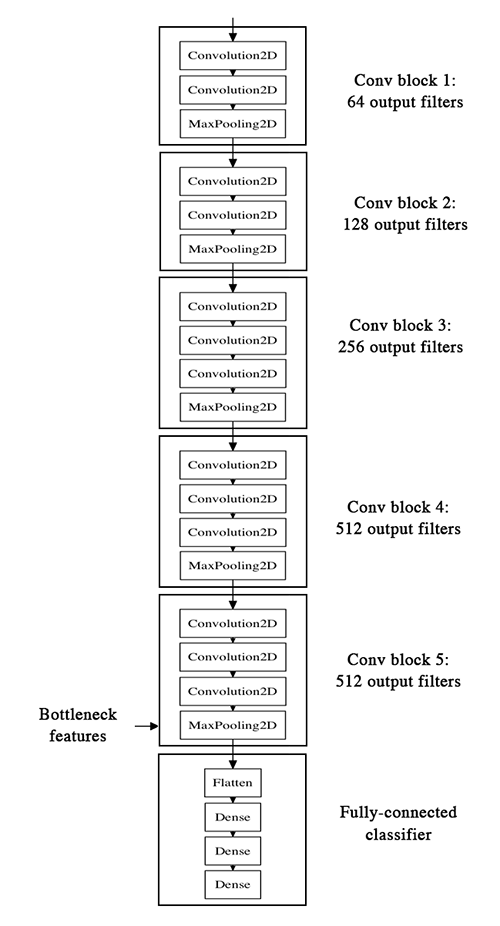
\includegraphics[scale=0.5]{img/vgg-architecture}
    \caption[]{VGG16 architektūros modelis\footnotemark}   % Antraštė įterpiama po paveikslėlio
    \label{img:vgg}
\end{figure}
\footnotetext{\url{https://blog.keras.io/img/imgclf/vgg16_original.png}}

\section{Inception-v3 architektūra}
\begin{figure}[H]
	\centering
	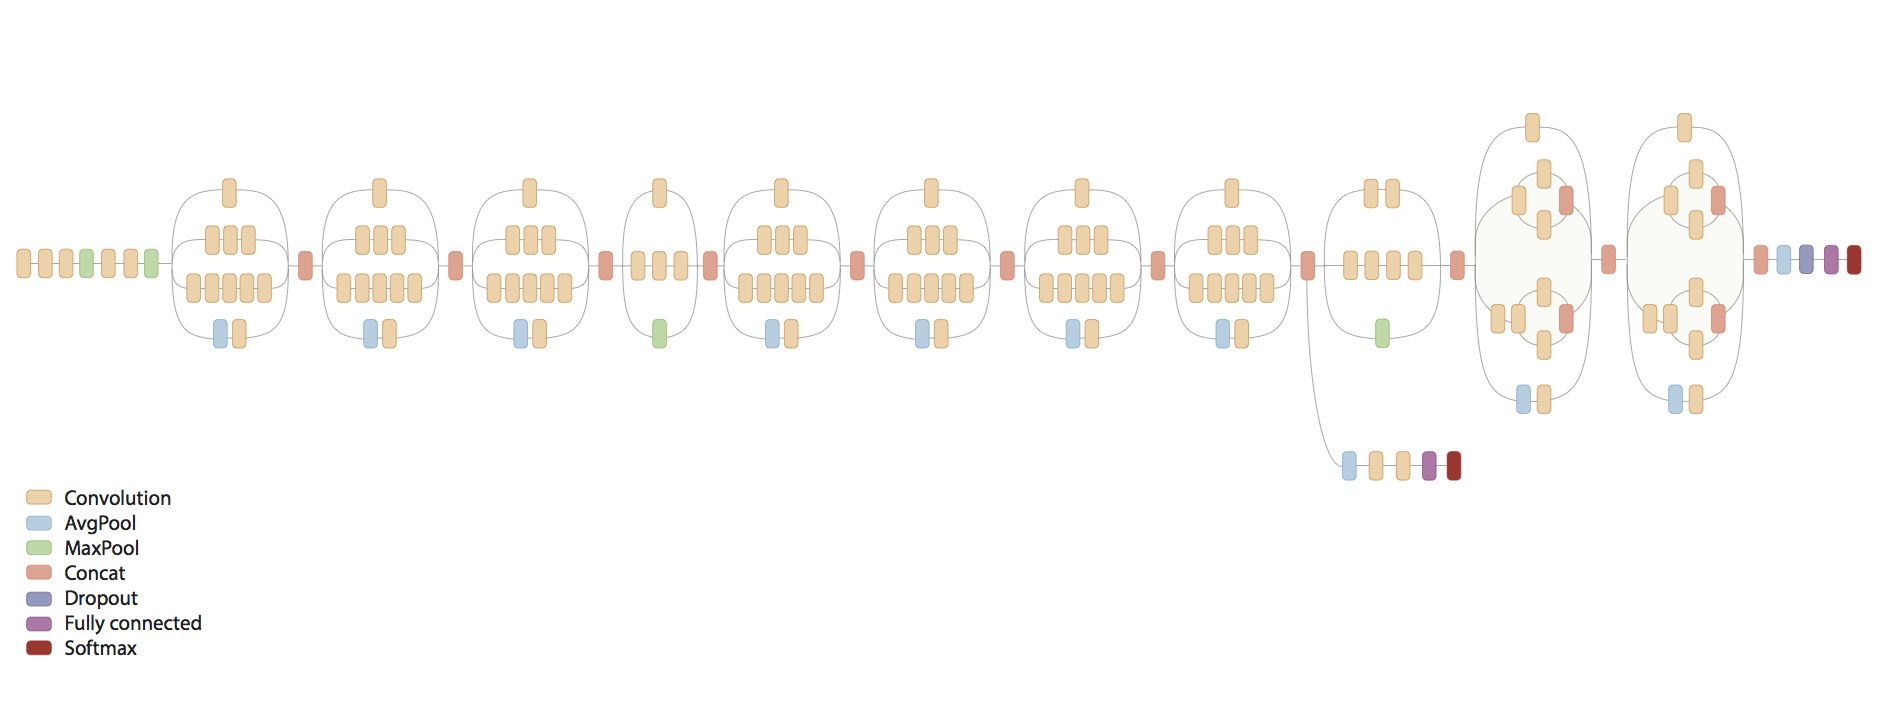
\includegraphics[scale=0.5]{img/inception_v3}
	\caption[]{Inception-v3 architektūros modelis\footnotemark}   % Antraštė įterpiama po paveikslėlio
	\label{img:inception}
\end{figure}
\footnotetext{\url{https://github.com/tensorflow/models/tree/master/inception}}
%
%
%\section{Eksperimentinio palyginimo rezultatai}
%% tablesgenerator.com - converts calculators (e.g. excel) tables to LaTeX
%\begin{table}[H]\footnotesize
%  \centering
%  \caption{Lentelės pavyzdys}    % Antraštė įterpiama prieš lentelę
%  {\begin{tabular}{|l|c|c|} \hline
%    Algoritmas & $\bar{x}$ & $\sigma^{2}$ \\
%    \hline
%    Algoritmas A  & 1.6335    & 0.5584       \\
%    Algoritmas B  & 1.7395    & 0.5647       \\
%    \hline
%  \end{tabular}}
%  \label{tab:table example}
%\end{table}

\end{document}
